\entry{Semana del 16/06/2025.}
\section{Lunes 16/06/2025.}
\subsection*{Configurar un Scan.}

Lo primero que hice fue pasar de leer un solo canal (donde nos habíamos quedado el Viernes pasado) a leer varios. Para esto se debe configurar los canales que serán medidos durante el Scan. En este caso fueron los canales 0 y 1 con las mismas flags que antes. Luego la función \textit{AdcRdScan} devuelve los valores de ese instante, y lo que hice fue un loop manual donde timeamos el tiempo que tarda cada uno.

% dev.AdcSetScan([0, 1], [gain, gain], [flags, flags])
\begin{lstlisting}
dev.AdcSetFreq(10000)

volts_data = []
timestamps = []
t_start = time.time()
	for i in range(iters):
	vals = dev.AdcRdScan(0, 1, gain, flags)
	data = np.array(vals)*max_voltage*2/(2**bit_depth) - max_voltage
	
	volts_data.append(data)
	timestamps.append(time.time() - t_start)

dev.Close()

\end{lstlisting}

Además setee la frecuencia de sampleo de cada canal como 10 kHz, para que la limitación del código fuese el loop (para lo que podemos compensar timeando cada iteración) y no la placa en sí. Nuevamente se deben convertir los valores binarios a voltaje. 

IMPORTANTE: En la función \textit{AdcRdScan} de \textit{daq.py} hay que corregir "flags[0]" por "wt.DWORD(flags)" para que funcione correctamente. 

\begin{figure}[th!]
	\centering
	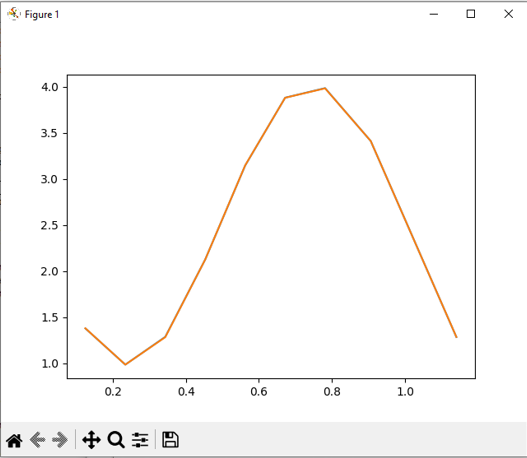
\includegraphics[width=0.415\linewidth]{Figures/09_06_2025/Scan_2_canales_manual}
	\caption{Scaneo manual de los canales 0 y 1 para el mismo output del generador de funciones (un seno de 1 Hz de frecuencia). El canal 0 está en azul por debajo y el 1 en naranja por arriba, pero coinciden casi que perfectamente así que no se nota.}
	\label{fig:scan2canalesmanual}
\end{figure}

Podemos ver que logramos medir ambos canales pero la frecuencia de sampleo deja bastante que desear, con lo cual el siguiente paso va a ser armar una adquisición continua a una frecuencia de sampleo determinada. 

Un par de cosas aprendidas sobre cómo funcionan los Scaneos en la placa. 
\begin{itemize}
	\item La devolución es un array de n valores, con n la cantidad de canales configurados. 
	\item La frecuencia de sampleo configurada es por canal siempre que sea posible, más sobre esto más adelante.
\end{itemize}

\subsection*{Armar una adquisición de N valores.}
Para esto seguí el procedimiento detallado en el Manual del Programador, ya que PyIOTech es solo un wrapper en python de lo que se explica ahí, pero mantiene en general los mismo nombres, argumentos, retornos, entre otras cosas. 

El código completo para leer N puntos de la placa es 

\begin{lstlisting}
N = 100

dev.AdcSetScan([0, 1], [gain, gain], [flags, flags])
dev.AdcSetFreq(10)
dev.AdcSetAcq(daqh.DaamNShot, 0, N)
dev.AdcSetTrig(daqh.DdtsImmediate, 0, 0, 0, 0)
dev.AdcTransferSetBuffer(daqh.DatmUpdateBlock | daqh.DatmCycleOff, N)
dev.AdcArm()
dev.AdcTransferStart()
dev.WaitForEvent(daqh.DteAdcDone)


vals = np.array(dev.dataBuf)
volts = vals * max_voltage * 2 / (2 ** bit_depth) - max_voltage

\end{lstlisting}

Este proceso se desglosa a continuación. 

\subsubsection*{Configurar escaneo.}
Se establece en \textit{AdcSetScan} los canales que serán leídos con los gains y flags correspondientes a cada uno. Acá usé las mismas flags y ganancia por X1 que veníamos usando desde antes. 

Luego se configura la frecuencia de adquisición deseada, esta va a ser la de cada canal siempre que sea posible. 

\begin{figure}[th!]
	\centering
	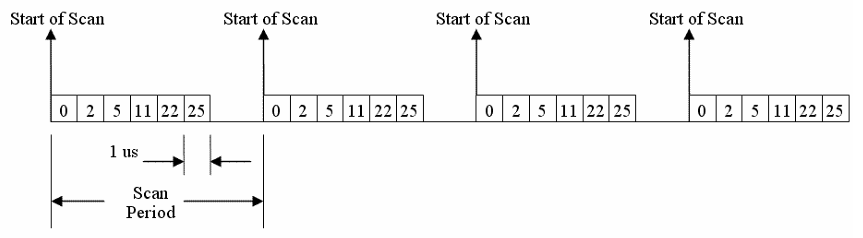
\includegraphics[width=0.567\linewidth]{Figures/09_06_2025/Tiempos_scan}
	\caption{Funcionamiento de la adquisición continua.}
	\label{fig:tiemposscan}
\end{figure}

El ADC es uno solo en la placa, y las mediciones de todos los canales del Scan se multiplexean para pasar por este, actuando a modo de cuello de botella. 

\begin{figure}[th!]
	\centering
	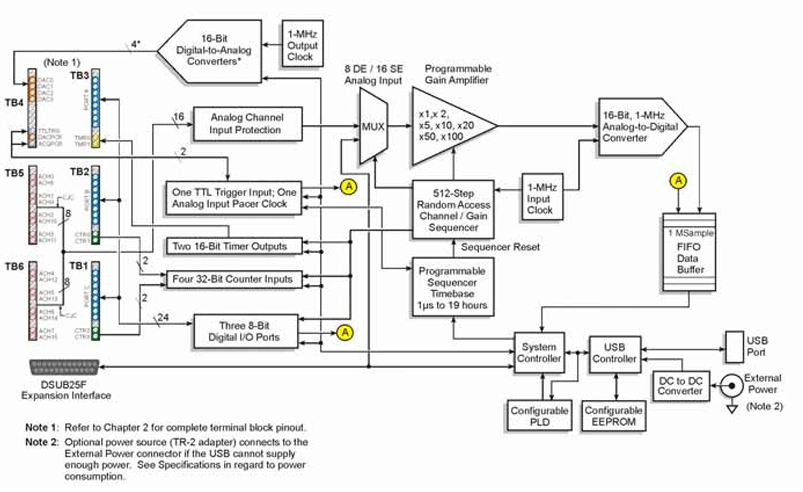
\includegraphics[width=0.5157146\linewidth]{Figures/09_06_2025/Diagrama_bloques_DAQ3000}
	\caption{Diagrama de bloques de la PSDAQ 3001.}
	\label{fig:diagramabloquesdaq3000}
\end{figure}

O sea, que la frecuencia máxima de sampleo es 1MHz agreggated, o sea, \textbf{distribuída entre todos los canales} del scaneo, no importan si son single-ended (que mide respecto del common) o differential gastan lo mismo del total (por eso conviene usar modo differential para que dos cuenten como uno solo). O sea, para dos canales, se debería poder samplear a un máximo teórico de 500 kHz cada uno. Además, cada canal necesita x tiempo para medirse, con lo cual esto va a limitar también la frecuencia máxima. En el esquema de arriba está marcado que cada canal tarda 1 $\mu$s en samplearse.

La placa después de \textit{AdcSetFreq} la ajusta para ser la máxima compatible. Se puede saber en cuánto quedó preguntando con \textit{AdcGetFreq}. 

\subsubsection*{Configurar adquisición.}
Configuradas las acciones a realizarse en cada escaneo ahora hay que configurar cómo va a funcionar la adquisición de los N escaneos que queremos. 

Con la línea: 
\begin{lstlisting}
dev.AdcSetAcq(daqh.DaamNShot, 0, N)
\end{lstlisting}
Estamos diciendo que va a durar N iteraciones (esa es la flag), con 0 disparos pretrigger y N postrigger, o sea, que todos se toman \textbf{después} del trigger.

Después configuramos el trigger para que sea inmediato al comienzo de la adquisición.

Finalmente debemos configurar el buffer que vamos a usar, donde se van a ir guardando los datos (en la computadora) a medida que los vaya mandando la placa. Como acá sabemos la cantidad de datos que va a mandar la placa, que serán n*N (canales por iteraciones), vamos a usar un buffer lineal con un tamaño prefijado.

\begin{figure}[th!]
	\centering
	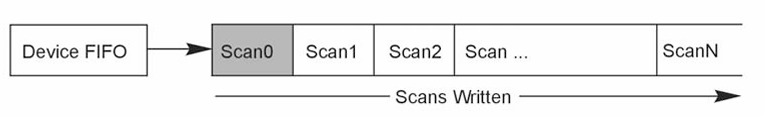
\includegraphics[width=0.7654\linewidth]{Figures/09_06_2025/Buffer_lineal}
	\caption{Esquema del funcionamiento del buffer lineal.}
	\label{fig:bufferlineal}
\end{figure}

\subsubsection*{Armar la adquisición.}
Armamos la adquisicón. A partir de este punto la placa va a estar esperando detectar el trigger para empezar a medir, en nuestro caso va a ser inmediato. 

La siguiente línea empieza la transferencia de datos, que se va a detener cuando se llene el buffer, aunque este no es el caso, la adquisición podría seguir pero no se escribirían más valores. 

Finalmente detenemos la adquisición y cerramos la comunicación con el dispositivo antes de procesar los datos. 

\subsubsection*{Procesado de los datos.}
Como ya habíamos dicho los datos van a estar en binario y va a haber que convertirlos a voltaje. En el buffer además los datos van a estar en el orden que se fueron midiendo, o sea, (canal 0, canal 1, canal 0, ..., canal 0, canal 1), con lo cual se deben separar teniendo esto en cuenta.

\begin{lstlisting}
max_voltage = 10.0
bit_depth = 16
def convert(vals):
	vals = np.array(vals)
	return vals * max_voltage * 2 / (2 ** bit_depth) - max_voltage
	
data = np.array(dev.dataBuf)
canal_1 = convert(data[::2])
canal_2 = convert(data[1::2])
tiempos = np.arange(iters)/freq
\end{lstlisting}

Más abajo una de las primeras adquisiciones que funcionaron.



\begin{figure}[!ht]
	\begin{minipage}[c]{0.5\textwidth}
			\begin{subfigure}{\textwidth}
					\centering
					\includegraphics[width=0.876\textwidth]{Figures/09_06_2025/Medición_100kHz.png}
					\captionsetup{width=0.8\textwidth}
					\subcaption{}
				\end{subfigure}
		\end{minipage}\begin{minipage}[c]{0.49\textwidth}
			\begin{subfigure}{\textwidth}
					\centering
					\includegraphics[width=0.876\textwidth]{Figures/09_06_2025/Medición_100kHz_zoom.png}
					\captionsetup{width=0.8\textwidth}
					\subcaption{}
				\end{subfigure}
		\end{minipage}
	\caption{Medición de señal de 1 Hz sampleando a 100 kHz en los canales 0 y 1. A la derecha se muestra un zoom, pero son virtualmente indistinguibles. El ruido que parece ser periódico por ahí son los 50/60 Hz de la pared, los cables no estaban muy prolijos.}
	\label{fig:medición_100kHz_y_zoom}
\end{figure}

\subsection{Máximo sampleo.}
Por último quise caracterizar el RLC con el que venimos trabajando, que tiene una frecuencia de unos 70 kHz. Al intentar samplear con este circuito a esa frecuencia estaba teniendo muy poca resolución de sampleo, y al usar el \textit{AdcGetFreq} resultó que para un canal estaba sampleando a un máximo de 200 kHz y para dos a un máximo de 100 kHz (siempre por canal). 

Pensé primero que la placa estaba limitando por algún motivo la frecuencia de sampleo, o bien que los diferenciales contaban como dos canales cada uno, que daría 250 kHz de sampleo máximo para 2, pero seguía siendo bastante más grande de lo que marcaba. 

\section{Miércoles 10/06/2025.}
No pudimos ir al Labo porque tomaron la decisión de tomar la Facultad y cerraron todos los ingresos a Ciudad Universitaria, excepto para tareas esenciales. 

\section{Resolución en frecuencia del Lock-in digital.}
Como parecía que íbamos a estar limitados a samplear a 100 kHz máximo estuve probando si con esa resolución el Lock-in de la semana del 31/03 funcionaría. En principio paar reconstruir una señal hay que samplear por lo menos a la frecuencia de Nyquist $f_n = 2*f_r$. Acá $f_r$ va a ser la de resonancia del RLC, y para lograr que sea menos de 50 kHz habría que aumentar C a 5 nF o más. 

Suponiendo que pudiésemos bajarla hasta 10 kHz y sampleando a 100 kHz nos interesa saber hasta qué frecuencia la reconstrucción de la modulación de fase va a ser fidedigna, ya que queremos que el sensor funcione a 1 kHz aproximadamente. Una buena forma de probar esto es generar una fase $\phi(t)$ que tenga contenido en frecuencia constante entre 0 Hz y 1 kHz y ver cómo la reconstruye el Lock-in a partir de samplear $A\sin(2\pi f_r + \phi(t))$.

Para construir $\phi$ usé: 

\begin{lstlisting}
T = 1.0
N = int(T*freq_sample) 

freqs = np.fft.rfftfreq(N, 1/freq_sample) 

spectrum = np.zeros_like(freqs, dtype=complex)
band = (freqs >= 0) * (freqs < f_max)
spectrum[band] = eps  * np.exp(2*np.pi*1j * np.random.rand(np.sum(band)))  

phi = np.fft.irfft(spectrum, n=N) * 2 * np.sqrt(N)
ts = np.linspace(0, T, N, endpoint=False)

\end{lstlisting}

Y al pasar por el lock-in con $f_{cutoff} = 1000$ Hz obtenemos:
	
\begin{figure}[!ht]
	\begin{minipage}[c]{0.5\textwidth}
		\begin{subfigure}{\textwidth}
			\centering
			\includegraphics[width=1.0990817\linewidth]{"Figures/09_06_2025/Límites del lockin sampleo y frecuencia"}
			\captionsetup{width=0.8\textwidth}
			\subcaption{$f_c=1$ kHz.}
		\end{subfigure}
	\end{minipage}\begin{minipage}[c]{0.49\textwidth}
		\begin{subfigure}{\textwidth}
			\centering
			\includegraphics[width=1.09918\textwidth]{"Figures/09_06_2025/Límites del lockin sampleo y frecuencia 2"}
			\captionsetup{width=0.8\textwidth}
			\subcaption{$f_c=5$ kHz.}
		\end{subfigure}
	\end{minipage}
	\caption{ Señal y FFT de la misma, original y reconstruída con el Lock-in para dos frecuencias de corte menores a $f_s$.}
	\label{fig:limites-del-lockin-sampleo-y-frecuencia}
\end{figure}

Notamos que hasta 750 Hz resuelve bastante bien y luego empieza a bajar. Creo que el decaimiento tiene más que ver con cómo elegir la frecuencia de corte (amplitud decae a la mitad en esta). Si elijo $f_c=5000$ Hz reconstruye completamente el espectro, así que sería factible usarlo en nuestro sistema bajo esta métrica.


También lo probé con cosenos o senos de una sola frecuencia y funcionaba bien bajo 1 kHz.

\section{Viernes 13/06/2025.}
\subsection*{Máximo Sampleo.}
Finalmente resultó que lo que estaba pasando es que cada canal estaba configurado por defecto para tardar 5 $\mu$s en ser medido, con lo cual bajaba la frecuencia máxima de sampleo del 1 MHz del ADC a 200 kHz. Esto se puede cambiar con la bandera "daqh.DafSettle1us". También se pueden usar "5us", "10us" y "1ms" si se quisiera. 

Con esto ya fue posible samplear a 1 MHz máximo en un solo canal, o 500 kHz en dos canales. 

\begin{figure}[th!]
	\centering
	\includegraphics[width=0.8017\linewidth]{"Figures/09_06_2025/Brrido 2 canales para señal de 100 kHz a 500 kS_s"}
	\caption{Addquisición en canal 0 y 1 del mismo output del generador de funciones (seno de 100 kHz).}
	\label{fig:brrido-2-canales-para-senal-de-100-khz-a-500-kss}
\end{figure}

Una cosa importante a considerar acá es que al estar sampleando al máximo posible tenemos que tener cuidado con los tiempos de cada medición, ya que el tiempo de la medición de cada canal es comparable con el tiempo de sampleo entre canales. Ya no podemos decir que ambas mediciones corresponden al mismo tiempo como cuando sampleábamos a frecuencias más bajas. Ahora va a haber 1 $\mu$s de delay entre el canal 0 y el 1, así que le sumamos ese delay a los tiempos del canal 1.\footnote{Antes también estaba este delay pero era muy bajo comparado con el tiempo entre un sampleo y el siguiente.}

\begin{lstlisting}
plt.plot(tiempos*1e6, canal_1, ".-", color="black", label = "Canal 1")
plt.plot((tiempos + 1e-6)*1e6, canal_2, ".-", color="orange", label = "Canal 2")

\end{lstlisting} 



Vemos que la señal medida por ambos canales sí es la misma, solo que la samplean en momentos distintos. Si graficamos el buffer crudo sin separar canales es como haber sampleado en un solo canal al doble de la frecuencia de adquisición, confirmando que efectivamente ambos miden la misma señal.

\begin{figure}[th!]
	\centering
	\includegraphics[width=0.65127\linewidth]{Figures/09_06_2025/Medición_2_canales_500kHz_sin_separar}
	\caption{Misma adquisición de la Figura \ref{fig:brrido-2-canales-para-senal-de-100-khz-a-500-kss} pero sin separar entre canal 1 y 2. Se nota que es un solo seno mejor definido.}
	\label{fig:medicion2canales500khzsinseparar}
\end{figure}


\subsection*{Armar una adquisición infinita.}
Lo siguiente a programar es la adquisición infinita, a diferencia de cuando tomamos solo N puntos, acá se pude dejar adquiriendo hasta que se desee frenar, o bien tomar una cantidad de puntos fijos pero muy grande, de forma tal que no sería eficiente tener un buffer lineal de ese tamaño en la memoria. 

El código final es el siguiente:
\begin{lstlisting}
dev.AdcSetScan([0, 1], [gain, gain], [flags, flags])
dev.AdcSetFreq(freq)
actual_freq = dev.AdcGetFreq()
print(f"Frecuencia de sampleo real por canal: {actual_freq} Hz.")

dev.AdcSetAcq(daqh.DaamInfinitePost, 0, 0)
dev.AdcSetTrig(daqh.DatsSoftware, 0, 0, 0, 0)
dev.AdcTransferSetBuffer(daqh.DatmUpdateBlock | daqh.DatmCycleOn, buf_size)
dev.AdcSetDiskFile(file_name, daqh.DaomCreateFile, 0)
dev.AdcArm()
dev.AdcTransferStart()
dev.AdcSoftTrig()

start_time = time.time()
timeout = 1.0 
acqTermination = False
while not acqTermination:
	dev.WaitForEvent(daqh.DteAdcData)  
	status = dev.AdcTransferGetStat()
	print(f"Transferidos: {status['retCount']} scans.")
	if time.time() - start_time > timeout:
		acqTermination = True

dev.AdcDisarm()
print(dev.AdcTransferGetStat())

\end{lstlisting}


\subsubsection*{Configurar el escaneo.}
Esto es igual que cuando tomamos N puntos. Se configuran los canales deseados.


\subsubsection*{Configurar adquisición.}
Ahora se usa "daqh.DaamInfinitePost" para establecer que no sabemos cuántos puntos vamos a tomar, se van a registrar hasta que se detenga en cierta condición. Ahora no importan la cantidad de puntos pos trigger ya que serán indefinidos. 

En este caso el trigger no va a ser inmediato sino que va a esperar a que el Software lo trigeree mediante "AdcSoftTrig".

Ahora el buffer va a ser circular en vez de lineal, ya que los datos se van a ir guardando en el disco se pueden ir reutilizando los espacios anteriores a modo de FIFO (First In - First Out). 


\begin{figure}[th!]
	\centering
	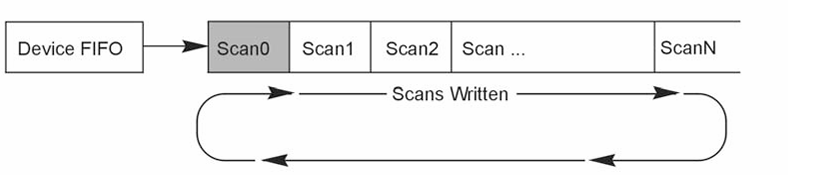
\includegraphics[width=0.78\linewidth]{Figures/09_06_2025/Buffer_circular}
	\caption{Esquema del buffer circular.}
	\label{fig:buffercircular}
\end{figure}

Es importante sin embargo que el buffer sea lo suficientemente grande, ya que el dispositivo acumula datos en su buffer interno y los manda de a tandas hasta donde entiendo, y que le dé tiempo a guardarse en el archivo. Si se recibe el error de "Buffer Overrun" durante la adquisición es bastante probable que sea porque el buffer era demasiado chico. Para samplear a 1 Mhz con un buffer de 50000 (o la función lo transforma en 100000 para 2 canales) parecería alcanzar.

Ahora establecemos en qué archivo se van a guardar los datos binarios (conviene guardarlos así, ya que convertidos serían floats que pesan más a priori). IMPORTANTE: Hay que cambiar en \textit{AdcSetDiskFile} "filename" por  ``ct.c\_char\_p(filename.encode('utf-8'))" para que funcione bien el nombramiento de los archivos, sino solo usaba la primera letra del string. % ´´ " 

La bandera de "daqh.DaomCreateFile" crea el archivo si no existe, pero si ya existe va a tirar error. Para sobreescribirlo habría que usar otra bandera.


\subsubsection*{Armar la adquisición.}
Se arma igual que antes la adquisición y se inicia la transferencia de datos, y se trigeree inmediatamente después en este caso.

\subsubsection*{Desarmar la adquisición.}
Mientras no haya pasado el tiempo establecido como condición para detener el escaneo se va esperando que haya data disposible en el driver buffer del dispositivo (con la flag "daqh.DteAdcData"), luego se irá transfiriendo al buffer de la computadora y escribiendo en el disco. 

Al final con \textit{AdcGetStat} se pregunta cuántos scans se trasnfirieron en total.  

\subsection*{Lectura de datos binarios.}
Después se puede leer el .bin y procesar los datos binarios como antes.

\begin{lstlisting}
binary_data = np.fromfile(filename, dtype=np.uint16)
    
\end{lstlisting}

El procesado será sensible a la frecuencia de sampleo y la cantidad de canales, como su configuración. Por esto es conveniente crear un archivo .json de metadata que contenga todo esto, como se hará más adelante.

\begin{figure}[th!]
	\centering
	\includegraphics[width=0.567\linewidth]{"Figures/09_06_2025/A disco directamente"}
	\caption{Adquisición directo a disco de muestra.}
	\label{fig:a-disco-directamente}
\end{figure}


\subsection*{Error handling.}
IMPORTANTE: Para que el printeo correcto de los errores que devuleve la DAQ hay que cambiar en la función "FormatError" de \textit{daq.py} el retorno de "msg.value" por "msg.value.decode(errors='replace')". % "" v Q 

\subsection*{Interfaz de usuario (GUI).} 
Con ayuda de ChatGPT armé una mínima GUI:

\begin{figure}[th!]
	\centering
	\includegraphics[width=0.457\linewidth]{Figures/09_06_2025/GUI_versión1}
	\caption{Primera versión de la GUI de adquisición de la placa.}
	\label{fig:guiversion1}
\end{figure}

Esta permite tomar mediciones ya sea fijas con un buffer lineal (modo "finito") o indeterminadas (modo "infinito"). También se pueden agregara canales, establecer la frecuencia de sampleo, el nombre del archivo donde se guardarán los datos (que para modo finito guarda el buffer al final del todo cuando se completa la medición) y en el caso de buffer circular determinar su tamaño. Por último en cualquiera de los modos se puede establecer ya sea el tiempo o la cantidad de iteraciones que se quieren tomar (aunque en el modo infinito va a ser un aproximado, y para 1 MHz lo mínimo son unas 8000 iteraciones por el tiempo que tarda en correr el código.) 

Alternativamente es posible poner en tiempo infinito un número muy grande y detener la adquisición manualmente cuando se desee con el botón correspondiente. 

También genera un archivo "filename\_metadata.json" que contiene la configuración de ese escaneo para su posterior lectura. 

Esta GUI viene acompañada de un código \textit{Formatter.py} con una función "read(filename)"que lee los archivos .bin y metadata.json y devuelve los tiempos y voltajes correspondientes a todos los canales medidos. % h 

\subsection*{Caracterización RLC.}
Haciendo uso de la interfaz se caracterizó el RLC que veníamos usando de C=561 pF, L=10 mH y R=1800 k$\Omega$. Fui barriendo con el generador varias frecuencias y tomando scaneos de 50000 puntos a la frecuencia máxima de sampleo. Primero se intentó con solo 5000 puntos pero el lockin no llegaba a resolver bien la amplitud y la fase (un ajuste por sinusoidales sí, pero la idea es usar el Lock-in para este tipo de cosas). El canal 0 es la referencia del generador y el canal 1 la caída de tensión sobre la resstencia, que debería ser proporcional a la corriente circulante por la Ley de Ohm. % á.  

\begin{figure}[th!]
	\centering
	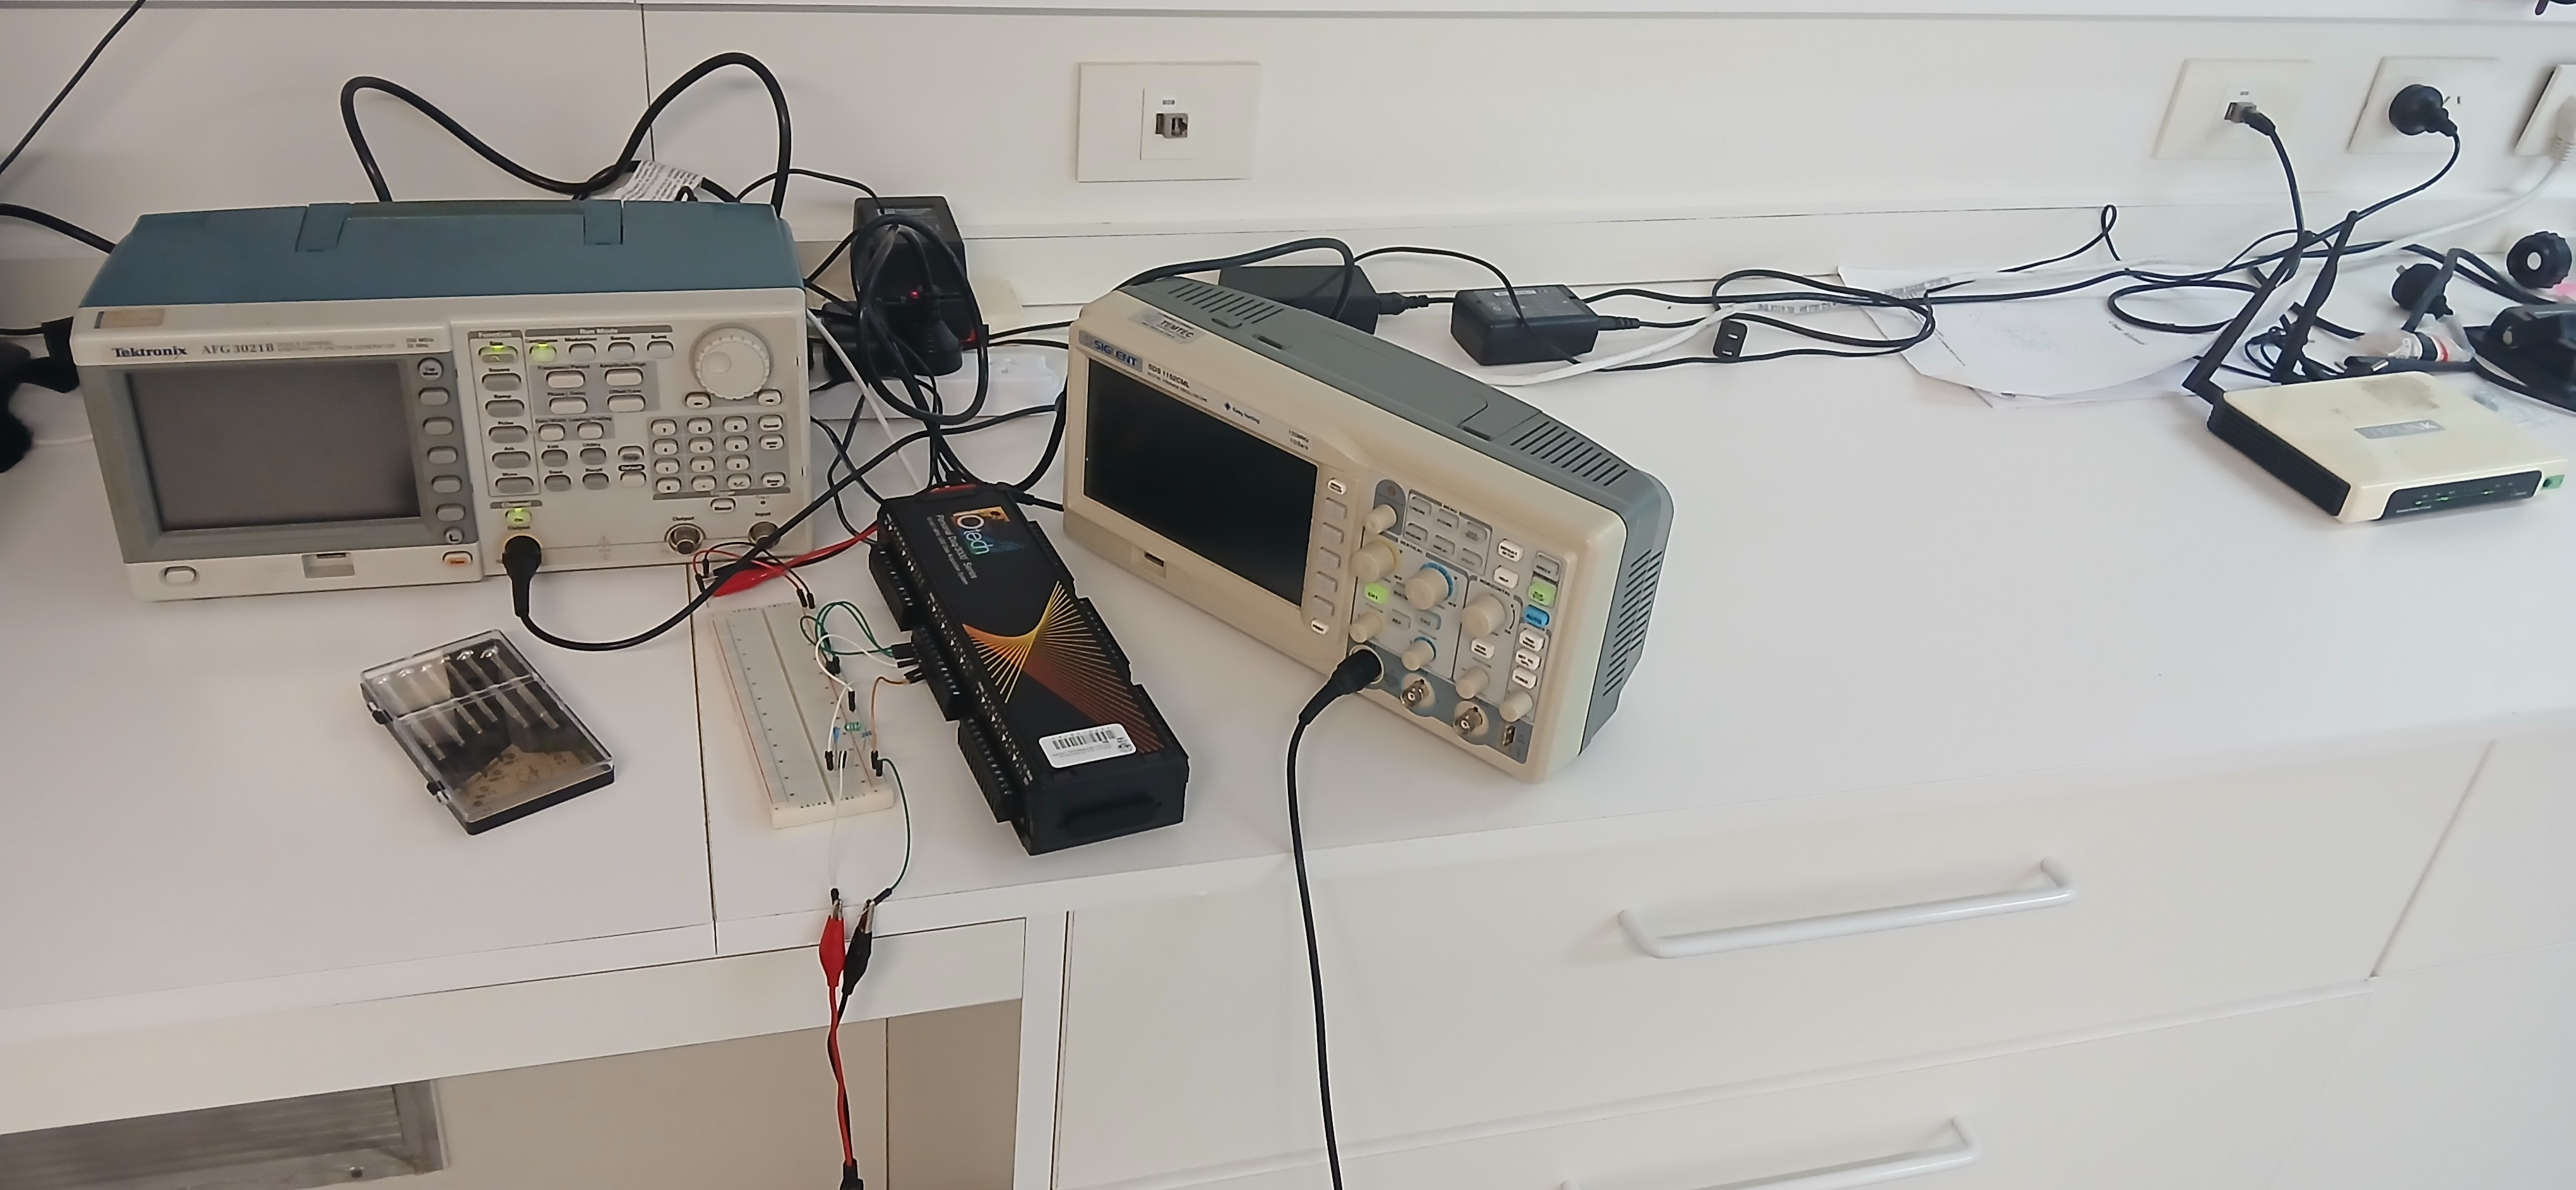
\includegraphics[width=0.567\linewidth]{Figures/09_06_2025/Setup_RLC}
	\caption{Setup para caracterizar el RLC con la placa.}
	\label{fig:setuprlc}
\end{figure}

Los resultados fueron los siguientes: 

\begin{figure}[th!]
	\centering
	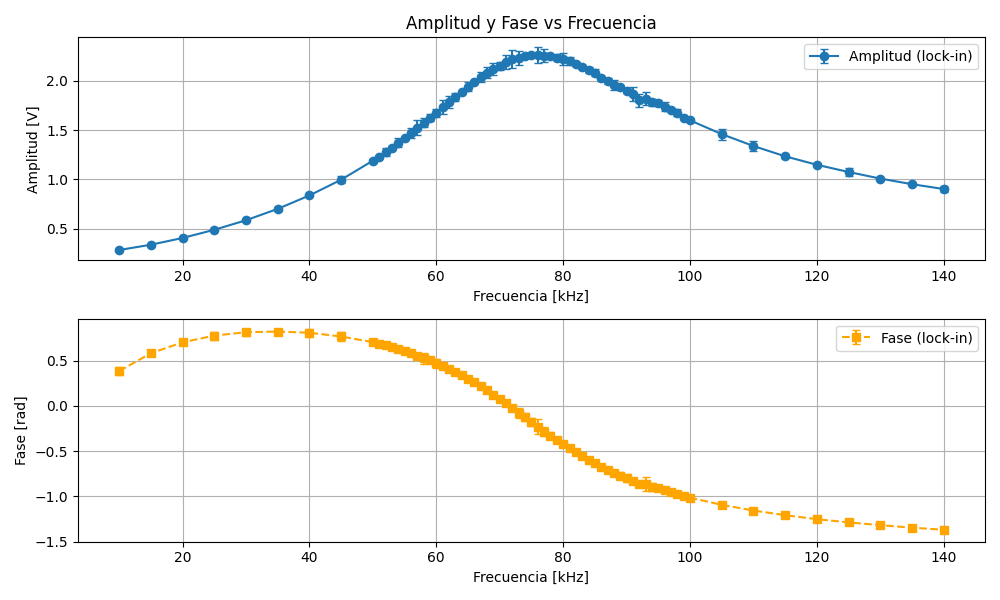
\includegraphics[width=0.87\linewidth]{Figures/09_06_2025/Barrido_RLC}
	\caption{Barrido de frecuencia del RLC.}
	\label{fig:barridorlc}
\end{figure}

El cómo se procesaron los datos para llegar a estos resultados se discute más adelante en la sección Lock-In Digital. Lo importante es que vemos la campana de resonancia con una frecuencia de unos 75 kHz donde la amplitud es máxima y la fase se hace 0°. % $ g o l a .

No parece irse a $+\pi/2$ cuando $f\rightarrow0$ pero podría ser por todos los cables que agregan capacitancias o algo así. 

\subsection*{Mediciones de prueba del sensor.} 
Para terminar el día con el tiempo que quedaba monté el sensor, conectando los alambres de cobre y acero al RLC ya conectado al generador de funciones y a la placa. Usé la cuba chica de 20x20 cm internos aproximadamente llena con agua destilada hasta una altura de 3.75 cm interna (medida con la regla de metal).

\begin{figure}[th!]
	\centering
	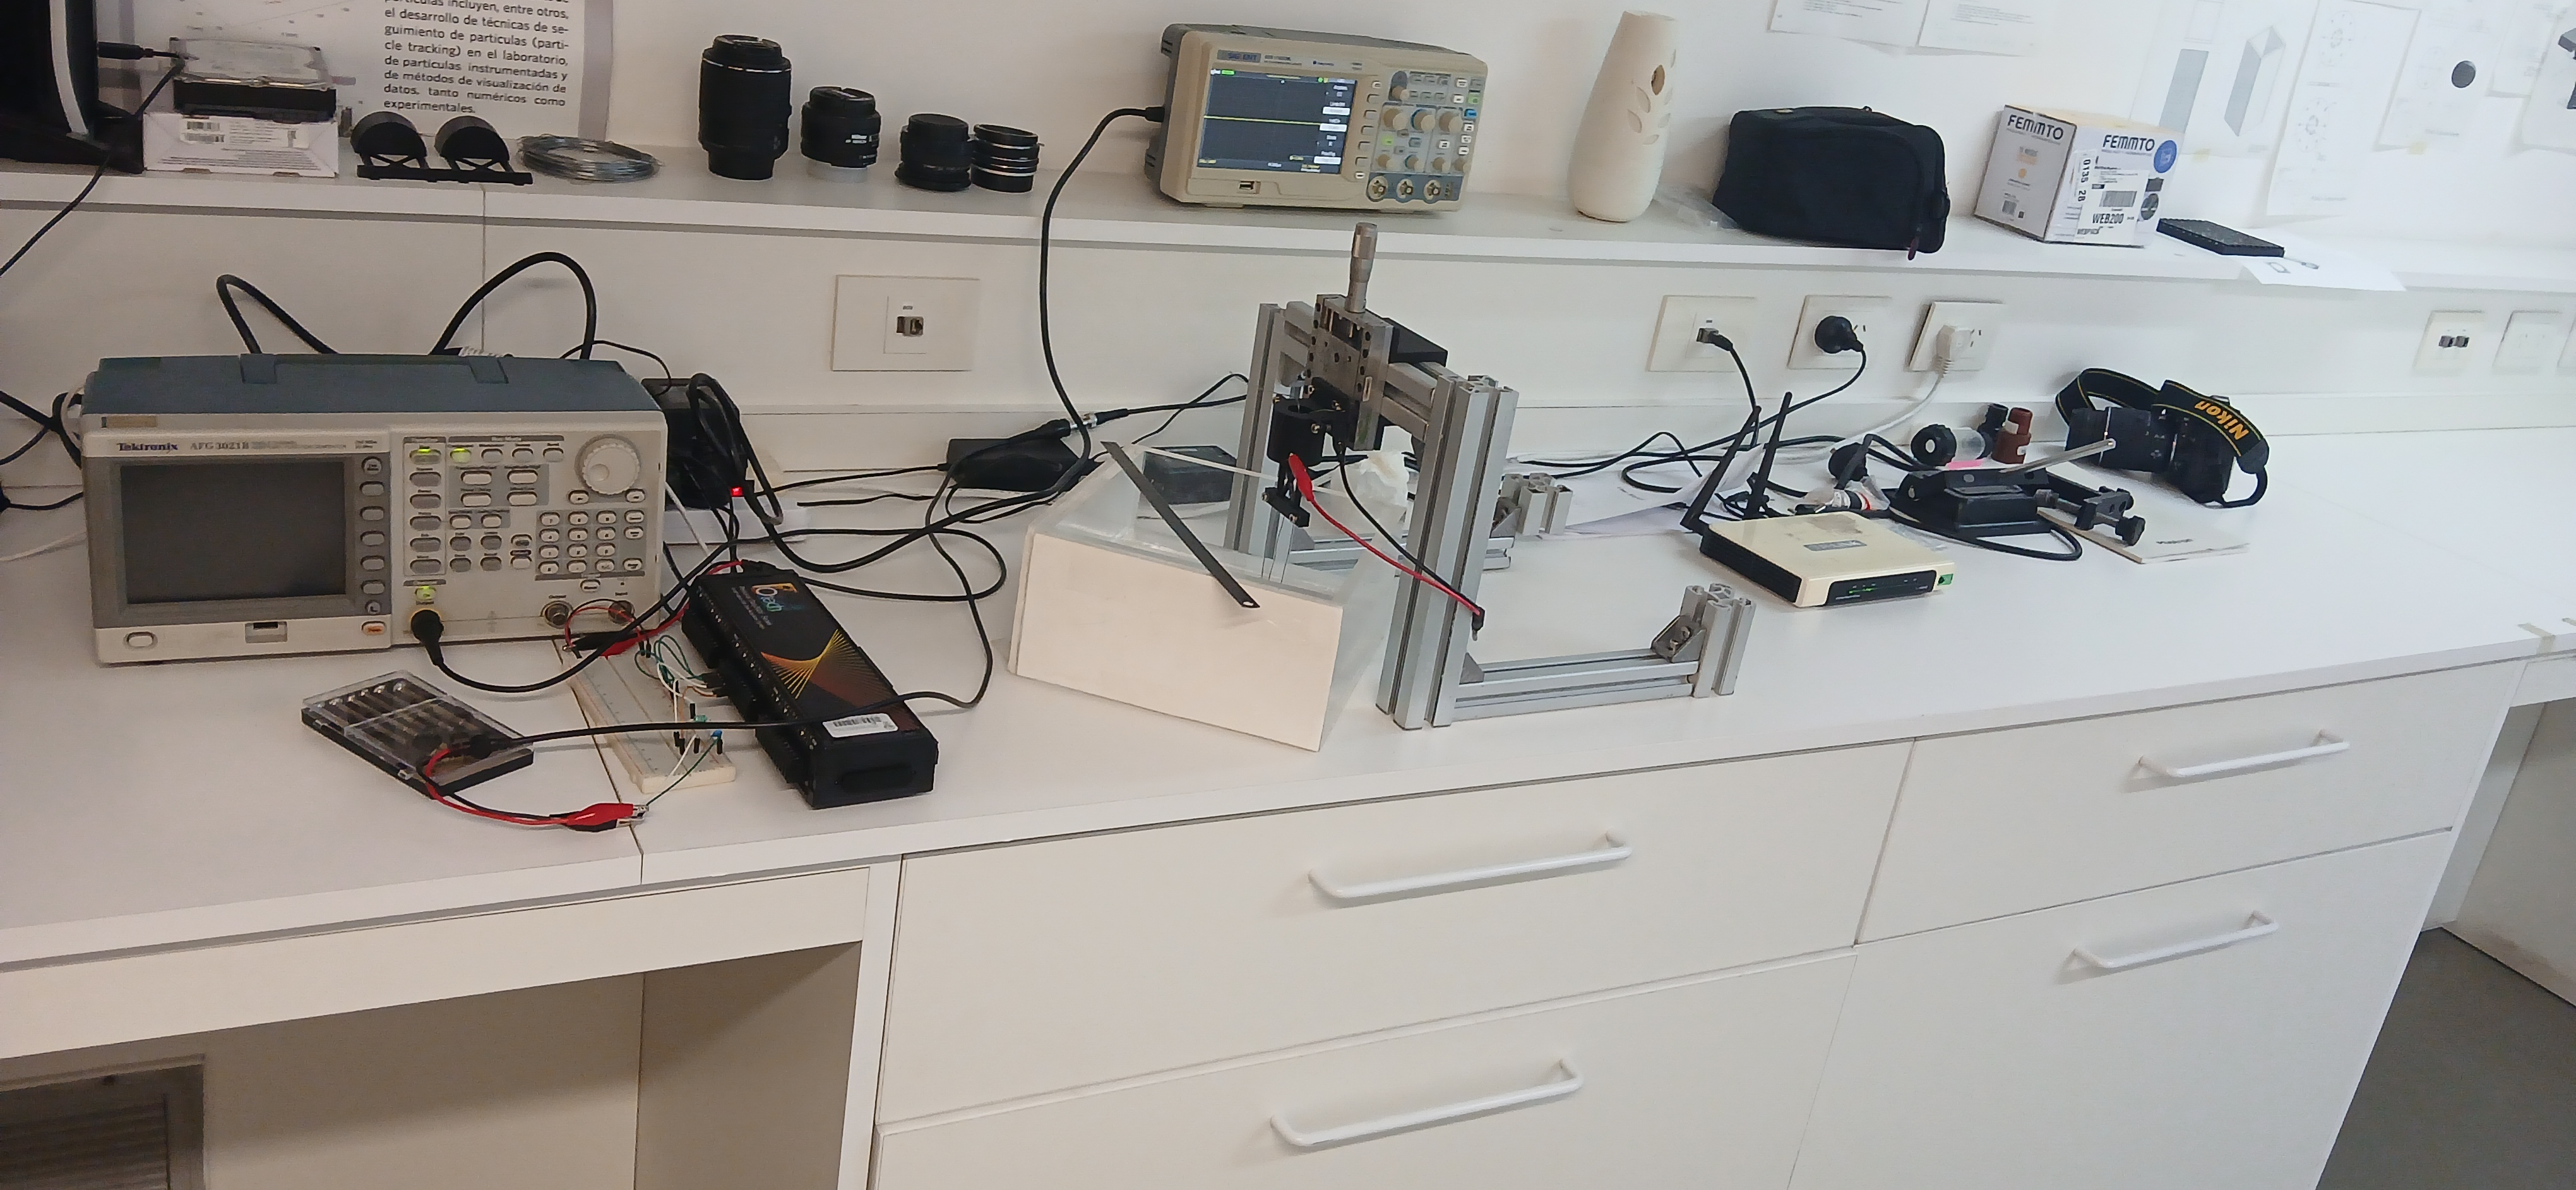
\includegraphics[width=0.567\linewidth]{Figures/09_06_2025/Setup_sensor}
	\caption{Setup para medir con el sensor y la placa.}
	\label{fig:setupsensor}
\end{figure}

Para poder usar el sensor tenemos que usar la nueva frecuencia de resonancia, que debería ser menor a 75 kHz ya que añadimos una capacitancia extra en paralelo al conectar el sensor sumergido. Estaría bueno medir la frecuencia de resonancia fuera del agua para saber cómo varía al sumergirlo. 

Repetí el barrido en frecuencias pero tomando solo 5000 puntos, con lo cual hay mayor error, especialmente en la amplitud. 

\begin{figure}[th!]
	\centering
	\includegraphics[width=0.87\linewidth]{Figures/09_06_2025/Barrido_RLC_más_Sensor}
	\caption{Barrido en frecuencia del RLC conectado con el sensor sumergido.}
	\label{fig:barridorlcmassensor}
\end{figure}

Por la posición donde la fase se hace 0° estimé que la nueva frecuencia de resonancia es 52 kHz. Así que para las últimas mediciones usé esa. No pude probar si cambiaba la fase al tocar la cuba u otras partes del setup. 

Tome varias mediciones de forzado y dejando caer gotas con la regla de metal, pero fueron de muy poca amplitud estas últimas. Un punto importante es que se salió un poco de agua antes de tomar las mediciones finales que voy a discutir más adelante.

\section{Lock-In Digital.}
Para poder aplicar el Lock-in de forma digital necesitamos los siguientes elementos:

\begin{itemize}
	\item Señal de referencia.
	\item Señal de interés con la fase modulada en el tiempo.
	\item Señal de referencia con shift de 90°. 
\end{itemize}

Todo evaluado en el mismo instante. Nosotros tenemos una pequeña desventaja, por la forma que adquirimos las señales tenemos la señal de referencia sampleada en $t_n$=0, 2, 4, ... $\mu$s y la de interés en $t_m$=1, 3, 5, ... $\mu$s. 

\begin{figure}[th!]
	\centering
	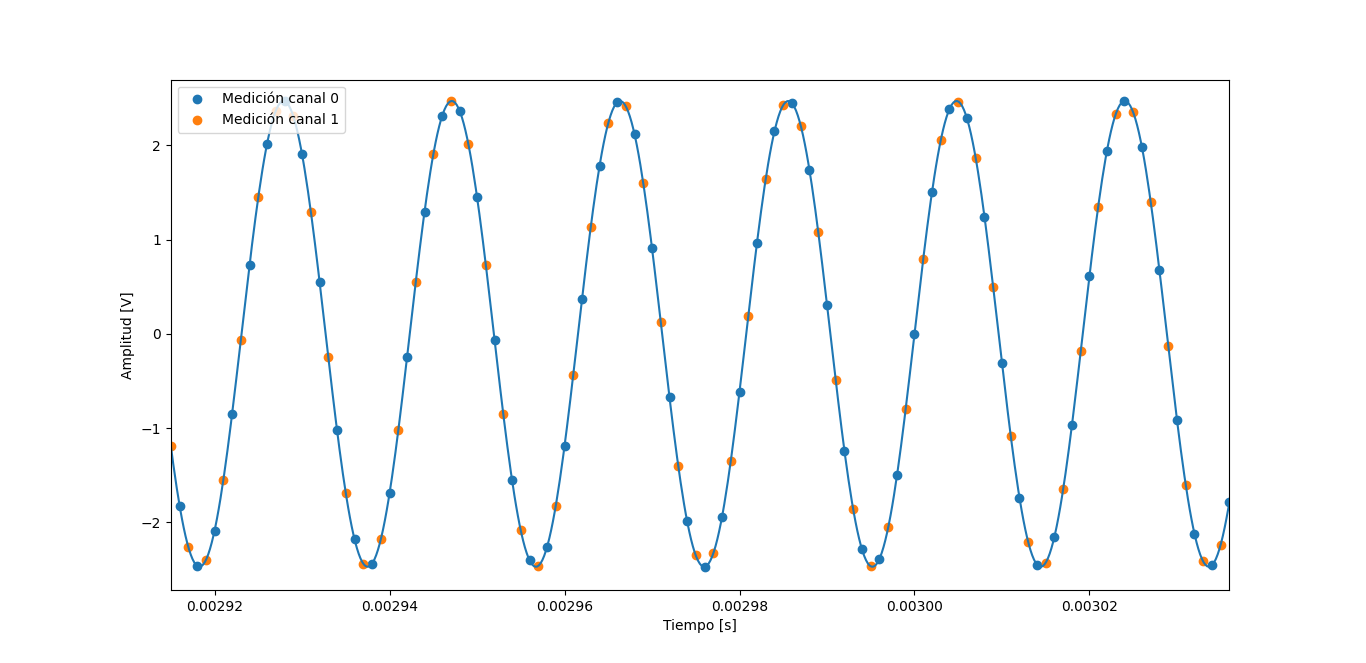
\includegraphics[width=0.87\linewidth]{Figures/09_06_2025/Sampleos2}
	\caption{Distintos momentos de sampleo entre canales para una señal de 52 kHz.}
	\label{fig:sampleos2}
\end{figure}

O sea, vamos a necesitar una forma de inferir el valor de la señal de referencia en los puntos que se muestrea la señal a analizar, ya sea por interpolación o alguna otra técnica. 

Además vamos a necesitar construir el coseno en esos mismos puntos de alguna forma. % $-

\subsection*{Ajuste senosoidal.} 
El primer enfoque para obtener la referencia sampleada en los puntos que necesitamos ($t_m$) fue ajustar los datos medidos (en $t_n$) para la referencia por:

\begin{equation*}
	Q_x(t_n) = A_0\sin(2\pi f_0 t_n+ \phi_0)
\end{equation*} 

Con parámetros $A_0$, $f_0$ y $\phi_0$. Luego la referencia resampleada y la señal shifteda 90° van a ser 

\begin{equation*}
	Q_x(t_m) = \text{sgn}(A_0)\sin(2\pi f_0 t_m+ \phi_0) \qquad \text{y} \qquad Q_y(t_m) = \text{sgn}(A_0)\cos(2\pi f_0 t_m+ \phi_0)
\end{equation*}

El signo es importante ya que sino sería como incorporar una fase de $\pm\pi$ aleatoriamente según si el ajuste da positivo o negativo, y esto daba lugar a tener que hacer unwrappings con periodo $\pi$ innecesarios.

Para pocos puntos este método funcionaba bastante bien, pero para las medidas de prueba con aproximadamente 13 millones de puntos por canal (para unos 25 segundos) ya no tanto. Los principales problemas de este método son los siguientes:

\begin{itemize}
	\item Durante mucho tiempo la señal de referencia no es perfectamente estable y va variando lentamente en el tiempo, lo que introduce ruido sino se tienen en cuenta durante el análisis. 
	\item Si el ajuste da una frecuencia levemente distinta a la real la fase va a tener sumando un término de la forma $\Delta\omega t$ que va a tener montada la fase que nos interesa y habría que hacer un detrend lineal. 
	\item El ajuste para muchos puntos lleva mucho tiempo. 
	\item Traté de limitar los parámetros para que $A_0$ siempre fuese positiva y $\phi_0$ vaya entre $[-\pi,+\pi]$ pero no encontraba parámetros óptimos por algún motivo. Y por defecto ``curve\_fit" de \textit{scipy} daba fases del orden de 50 radianes. 
\end{itemize}

Para evitar estos problemas traté de analizar los datos de a ventanas que se solapen, quedándome con la última mitad de los datos, ya que el lock-in siempre hace cosas raras con los primeros puntos. Pero hacia los últimos datos siguen apareciendo las tendencias lineales en la referencia y no estoy muy seguro porqué (incluso analizando referencia contra referencia). No sé si serán los últimos datos antes de detener la medición o si a partir de 20 segundos de medir pasa algo, como se ve más abajo (para medición de forzado diagonal del tanque y relajación, después de que se salió un poco de agua). 

\begin{figure}[th!]
	\centering
	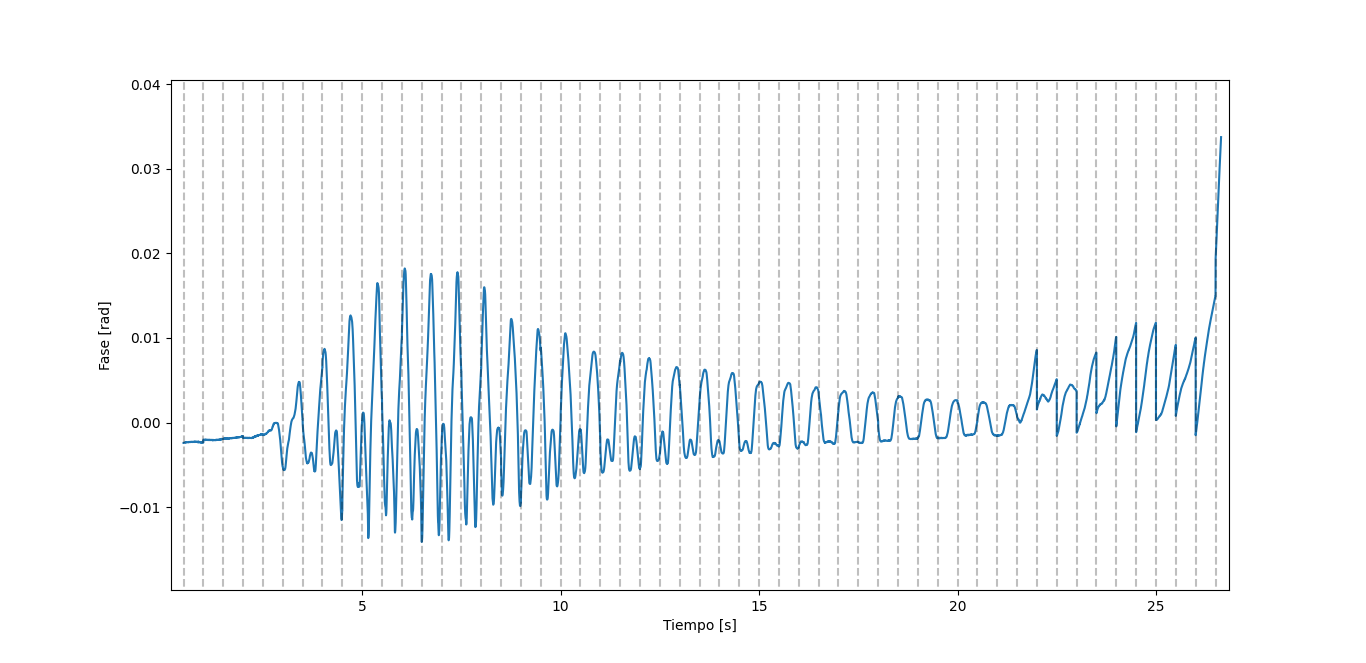
\includegraphics[width=0.857\linewidth]{Figures/09_06_2025/Lock_in_ajuste_intervalos_con_overlap}
	\caption{Método de reconstrucción de la señal de referencia por ajuste de cuadrados mínimos en intervalos con overlap de la señal.}
	\label{fig:lockinajusteintervalosconoverlap}
\end{figure}

Por otro lado haciendo el ajuste en la señal completa imagino que se compensan los errores en la señal de referncia pero igual queda un pequeño ruido que hay que restar a posteriori (por ahí si la amplitud de la fase fuese mayor no se notaría tanto).

\begin{figure}[th!]
	\centering
	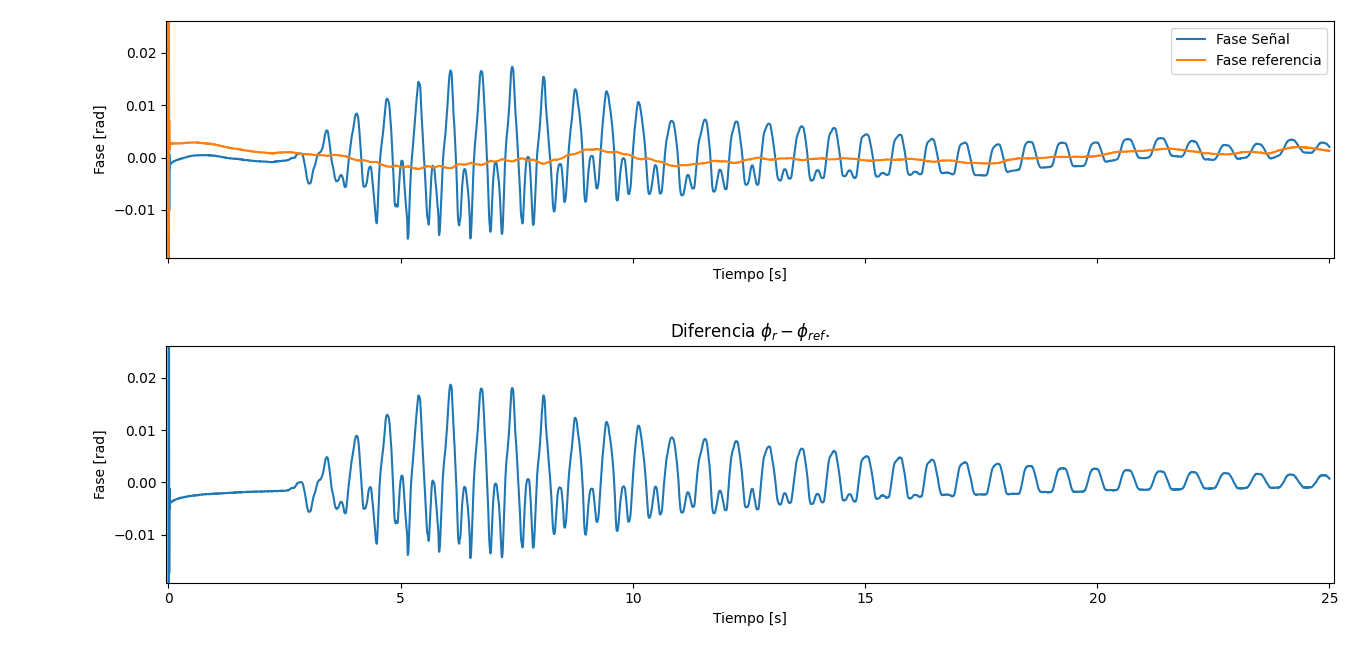
\includegraphics[width=0.987\linewidth]{Figures/09_06_2025/Lock_in_ajuste_completo}
	\caption{Lock in de la medición completa con reconstrucción de la referencia por Ajuste de cuadrados mínimos.}
	\label{fig:lockinajustecompleto}
\end{figure}

Con esto queda funcionando el método, pero hay que hacer dos veces el análisis (una para la señal y otro para la referencia) lo que no es del todo muy eficiente.


\subsection*{Fractional delay.} 
Otra opción para reconstruir la referencia es utilizar lo que se conoce como \textbf{Fractional Delay Filters}. Estos nos permiten para una señal con un ancho de banda limitado, tal que esa frecuencia máxima sea sampleada regularmente a la frecuencia de Nyquist. \cite{roelandtsHowCreateFractionalDelay2019}

Esto se debe a la aplicación del Teorema de Whittaker–Shannon que nos permite reconstruir ese tipo de señales completamente. Supongamos que tenemos $Q[n]$ sampleada en los puntos $t_n$. Entonces la señal completa va a ser:

\begin{equation}
	Q(t) = \sum_{n=-\infty}^{+\infty} Q[n]\text{sinc}\left(\frac{t-nT}{T}\right) \qquad \text{con} \qquad \text{sinc}(t) = \frac{\sin(\pi t)}{\pi t}
\end{equation}

Con $T=1/f_s$. Por simplicidad consideremos $T=1$ ya que vamos a agregar un delay no cambia. Luego si queremos retrasar la señal una fracción $j=\tau/T$, entonces vamos a tener la señal evaluada en $t=t_m-\tau$ o $t/T=m-j$

\begin{equation}
	Q[m-j] = \sum_{n=-\infty}^{+\infty}Q[n]\text{sinc}(m-j-n)
\end{equation} 

Y si recordamos la definición de la convolución discreta:

\begin{equation}
	Q[m-j]=(Q*h)[m] = \sum_{n=-\infty}^{+\infty}Q[n]h[m-n] \qquad \text{con} \qquad h[n]=\text{sinc}(n-j)
\end{equation}

Acá sin embargo tenemos una sumatoria infinita y el sinc($x$) no decae a 0, no tiene soporte finito, y la cantidad de datos que podemos medir son limitados. Así que para solucionar esto usamos una ventana que lo lleve a 0 en cierta cantidad de puntos, cuantos más usemos mejor funcionará ya que más términos tiene la sumatoria. 

En python queda:

\begin{lstlisting}
def resample(ts, signal):
	fs = 1/(ts[1] - ts[1-1])
	t0 = -0.5
	h = fractional_delay(t0)
	delayed = convolve(signal, h, mode="same")
	new_ts = ts - t0/fs
	return new_ts, delayed
	
def shift_90(ts, signal):
	fs = 1/(ts[1] - ts[1-1])
	
	Ar, fr = fft_parameters(ts, signal)
	
 	Delta = -1/4 * fs/fr 
	h_cos = fractional_delay(Delta)
	cos_measured = convolve(signal, h_cos, mode="same")
	return cos_measured
\end{lstlisting}


Donde obtenemos los coeficientos del FDF con la librería de \textit{pyroomacoustics}:

\begin{lstlisting}
def fractional_delay(t0):	
	N = constants.get("frac_delay_length")
	
	if isinstance(t0, np.ndarray) and t0.ndim == 1:
	t0 = t0[:, None]
	
	return np.hanning(N) * np.sinc(np.arange(N) - (N - 1) / 2 - t0)
	
\end{lstlisting}

El N=81 por defecto y usa la ventana Hanning. Parece estar funcionando bastante bien. Para el seno hay que retrasar medio punto de sampleo y a parte correr los tiempos. Para el coseno hay que retrasar un tiempo que de una fase de 90°:

\begin{equation}
	2\pi f \Delta t = \pi/2 \quad \Rightarrow \quad \Delta t = j/f_s = 1/(4f) \quad \Rightarrow \quad j = f_s/(4f)
\end{equation}

Y luego de retrasarla 90° resamplearla para que esté en los mismos puntos que la señal original de interés. Ahora que lo pienso se podría retrasar 90° directamente el seno resampleado. 

\begin{figure}[th!]
	\centering
	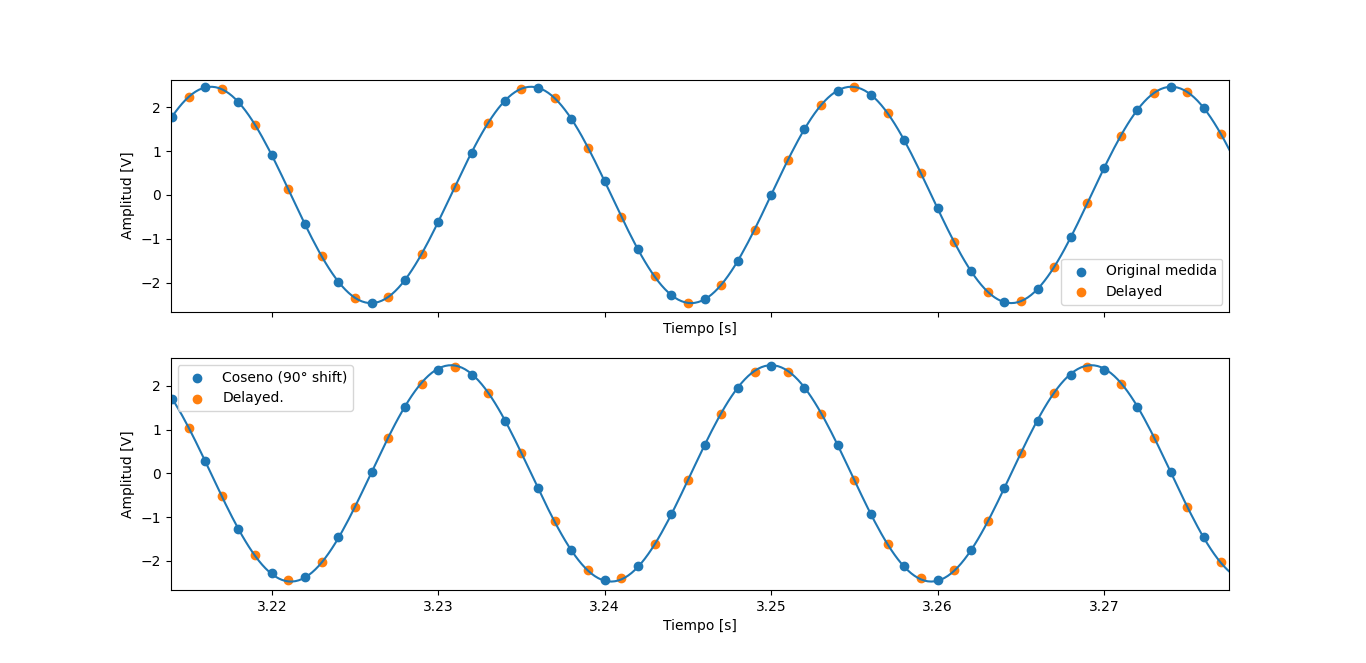
\includegraphics[width=0.87\linewidth]{Figures/09_06_2025/Fractional_Delay}
	\caption{Resampleo de una señal artifical y shifteo de 90° con los FDF.}
	\label{fig:fractionaldelay}
\end{figure}

Con esta reconstrucción de las señales de referencia se puede hacer el Lockin a toda la señal completa (13 millones de puntos) y es bastante más rápido. 

\begin{figure}[th!]
	\centering
	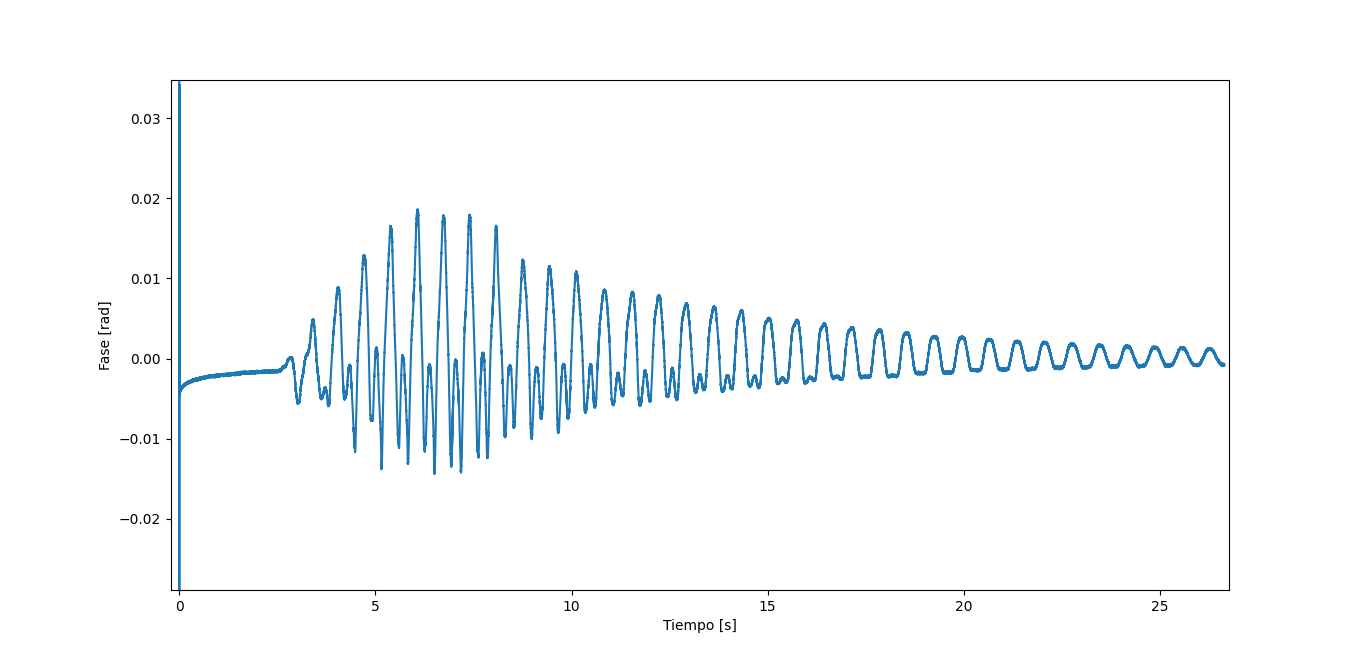
\includegraphics[width=0.987\linewidth]{Figures/09_06_2025/FDF_completa}
	\caption{Señal completa analizado con el lock in y FDF.}
	\label{fig:fdfcompleta}
\end{figure}

Y acá además no hace falta analizar la referencia por separado porque se usa la verdadera punto a punto y no una artificial como antes.

Además tarda para analizar 50000 puntos (0.1 s a 500 kHz de sampleo) en 0.015 s con lo que se podrpia usar a tiempo real sampleando un poco menos, por ejemplo, durante 0.085 s, y tener 10 puntos por segundo.

\subsection*{Filtro exponencial.}
Por último, vine usando hasta ahora el butter low pass filter para el lock-in, pero en \cite{harvieOLIAOpensourceDigital2023} usan uno que se conoce como filtro exponencial o exponential moving average, tal vez más conveniente para tiempo real, ya que solo depende de los puntos anteriores. Si tenemos nuestros valores en un determinado momento:

\begin{equation}
	X_0[n] = A[n]C[n] \qquad \text{y} \qquad Y_0[n] = A[n]S[n]
\end{equation}

Con $A[n]$ la señal de interés con la modulación, $S[n]$ la referencia (para esto el seno) y $C[n]$ la shifteada 90°, el coseno. Luego filtramos en dos etapas, usando el parámetro $\alpha=\cos(\gamma)-1+\sqrt{\cos^2(\gamma)-4\cos(\gamma)+3}$ que se relaciona con la frecuencia de corte o el tiempo de integración $\tau$ de la forma: $\gamma=2\pi f_c/f_s$ con $f_s$ la frecuencia de sampleo. Entonces:

\begin{align}
	X_1[n] &= X_1[n-1] + \alpha(X_0[n]-X_1[n-1]) \\
	Y_1[n] &= Y_1[n-1] + \alpha(Y_0[n]-Y_1[n-1]) \\
\end{align}

y la segunda etapa: 

\begin{align}
		X_2[n] &= X_2[n-1] + \alpha(X_1[n]-X_2[n-1]) \\
		Y_2[n] &= Y_2[n-1] + \alpha(Y_1[n]-Y_2[n-1]) \\
\end{align}

Y podemos elegir trivialmente $X_0[-1]=Y_0[-1]=0$. Con este para la señal anterior y el FDF tenemos: 

\begin{figure}[th!]
	\centering
	\includegraphics[width=0.987\linewidth]{"Figures/09_06_2025/Exponential filter más FDF"}
	\caption{Filtro exponencial + FDF de la señal completa.}
	\label{fig:exponential-filter-mas-fdf}
\end{figure}


También funciona bastante bien, pero para el array ya entero funciona un poco más lento que el butter low pass de antes. Para tiempo real no lo sé todavía.  

Con el ajuste de nuevo habría que restar la fase de la referencia original. 


\section*{Análisis espectral.} % sub 
Por último el mismo análisis espectral que ya hicimos para el SR830.

\begin{figure}[th!]
	\centering
	\includegraphics[width=0.987\linewidth]{"Figures/09_06_2025/Análisis espectral señal frozado"}
	\caption{Análisis espectral forzadao y relajación.}
	\label{fig:analisis-espectral-senal-frozado}
\end{figure}

De nuevo la fundamental es la más excitadas pero después aparecen múltiplos de la misma y no sé del todo porqué, por ahí las no linealidades del sistema afectan acá.